\section{Versuchsaufbau}

\begin{figure}[h!]
	\centering
	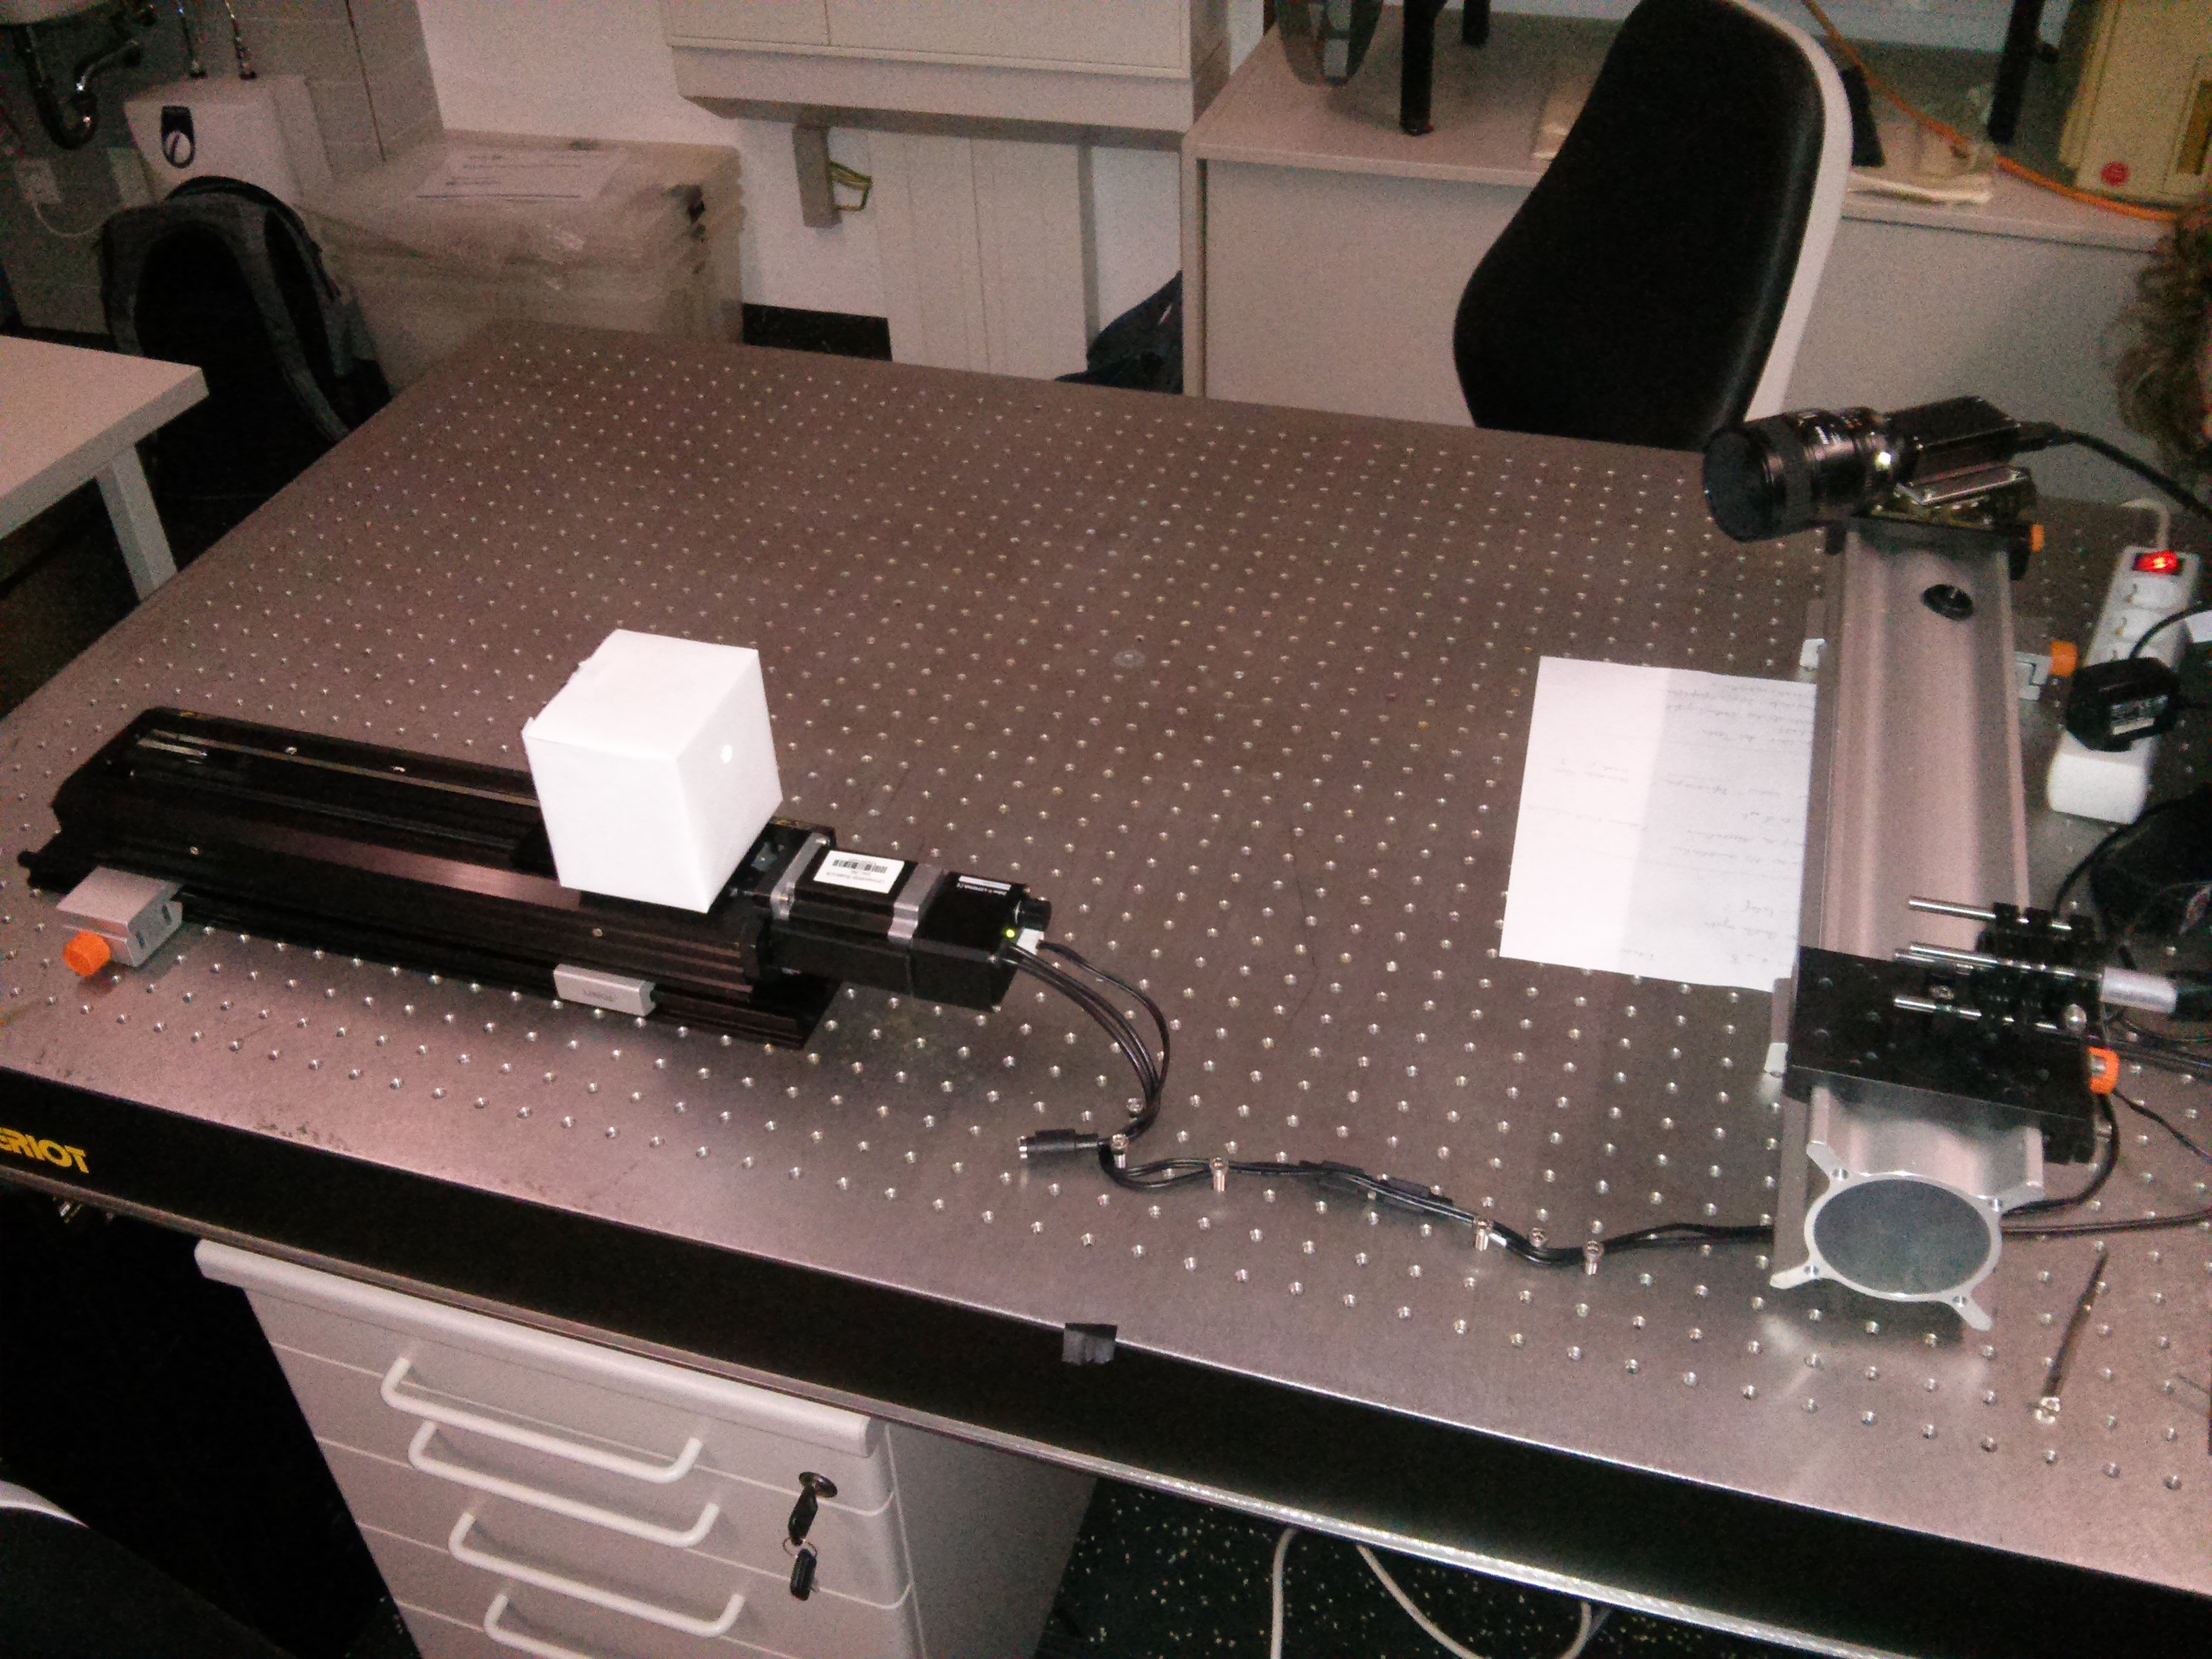
\includegraphics[width=0.8\linewidth]{img/versuchsaufbaufoto.jpg}
	\caption{Versuchsaufbau}
	\label{fig:Versuchsaufbau}
\end{figure}

Der Versuchsaufbau bestand aus insgesamt drei voneinander örtlich getrennten Komponenten. 

Die Komponenten des zu vermessenden Systems, bestehend aus einem grünen $532 \si{\nano\meter}$ Laser (Neodym-dotierter Yttrium-Aluminium-Granat-Laser (Nd:YAG)) und einem Messobjekt, sind in einer Linie angeordnet. Dieses Messobjekt hat die Form eines Würfels. Die Oberfläche dieses Würfels ist mit weißem Papier umspannt, um den Laserpunkt gutsichtbar abzubilden. Der Würfel konnte mittels einer Linearachse (Zaber T-LST0250 A) mit einer Genauigkeit von $0.124023438 \si{\micro\meter}$ in z-Richtung verschoben werden. Der Schrittmotor der Linearachse konnte mithilfe des angeschlossenen PCs angesteuert werden.

Das beobachtende System bestand aus einer Kamera (Basler Scout scA1400-36fm) mit einem $60 \si{\milli\meter}$ Nikon Objektiv. Die erfassten Bilder wurden direkt an den angeschlossenen PC zur weiteren Verarbeitung übertragen.

Die Auswertung der im Versuch aufgenommenen Bilder erfolgte auf einem direkt an die Komponenten des Versuchsaufbaus angeschlossenen PCs mithilfe der Software Mathcad.

Um auf den aufgenommenen Bildern Störlichtquellen abzuschirmen musste Tino dauerhaft vor einer Steckerleiste stehen, bis er diese einfach abschaltete $\ddot\smile$